%%
% ----------------------------------------------------------------------------
% "THE BEER-WARE LICENSE" (Revision 42):
% <sebastian.rauh@hs-heilbronn.de/michael.bauer@hs-heilbronn.de> wrote this 
% file. As long as you retain this notice you can do whatever you want with 
% this stuff. If we meet some day, and you think this stuff is worth it, you 
% can buy us a beer in return. 
% Michael Lukas Bauer, Sebastian Felix Rauh
% ----------------------------------------------------------------------------
%%

Die in Kapitel 3 aufgeführten Analyse Ergebnisse wurden für die erste Interation des Prototyps umgesetzt. Es handelt sich hierbei um ein funktionsfähigen Prototypen, der nativ auf der Apple Watch ausführbar ist. Im folgenden werden Schritte der Umsetzung genauer beschrieben. Hierbei wird genauer auf die Benutzeroberflächenerstellung, sowie auch die Verbindung zischen Uhr und iPhone eingegangen.

\section{Benutzeroberfläche}
Xcode bietet für visuelle Erstellung von Benutzeroberflächen ein eigenen integrierten Editor namens InterfaceBuilder bereit. Hiermit können graphische Elemente per DragAndDrop zu einer Benutzeroberfläche zusammengestellt werden \ref{fig:xcode-interface-elements}. Ebenfalls per DragAndDrop werden diese Inerface-Elemete mit dem Quellcode verbunden\ref{fig:xcode-interface-code-connect}.

Die Auswahl an Interface-Elemenete ist sehr begrenzt und bietet kaum Möglichkeiten eigene Interface-Elemenete zu erstellen. Trotz dieser Begrenztheit lassen sich Anwendungen komplexere Anwendungen bauen. 
\begin{figure}
	\caption{Interface Elemente zu Erstellen von Benutzeroberflächen}
	\label{fig:xcode-interface-elements}
	\centering
		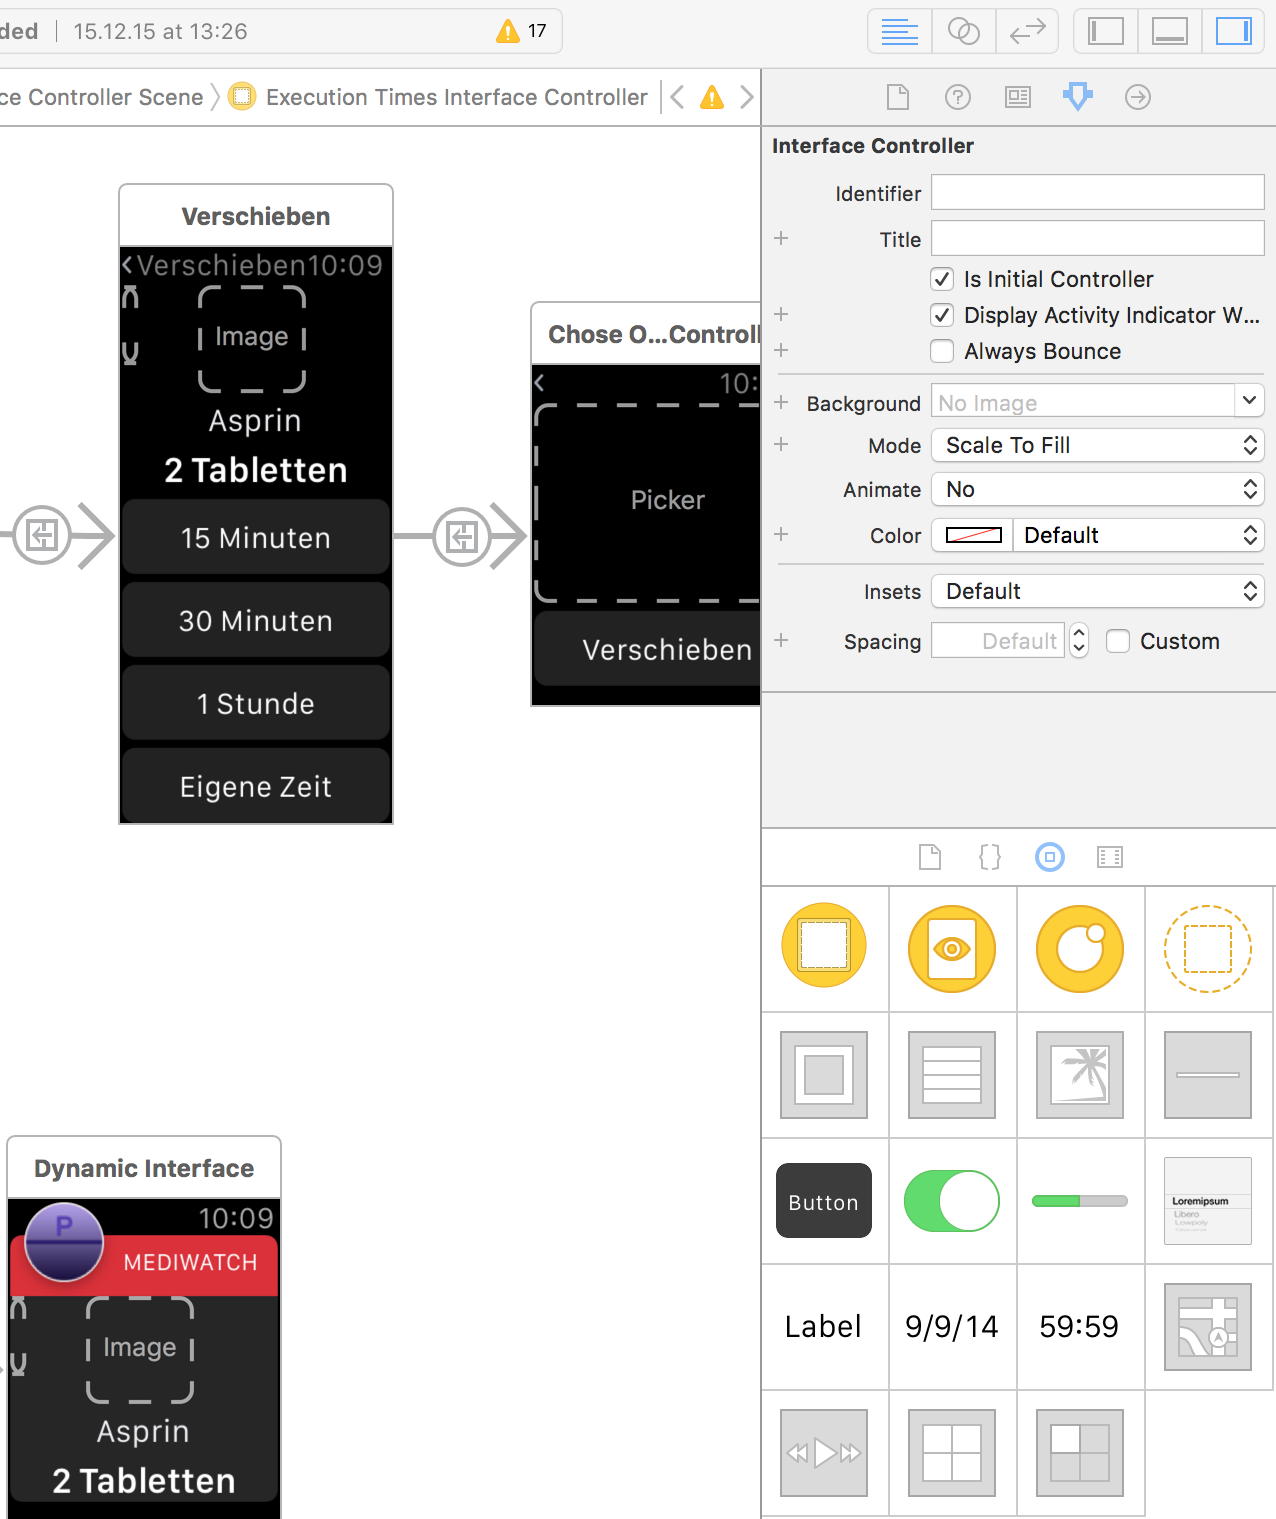
\includegraphics[width=0.9\textwidth]{04_realisation/screenshots/xcode-interface-elements}
\end{figure}

\begin{figure}
	\caption{Interface Elemente mit Quellcode verknüfen}
	\label{fig:xcode-interface-code-connect}
	\centering
	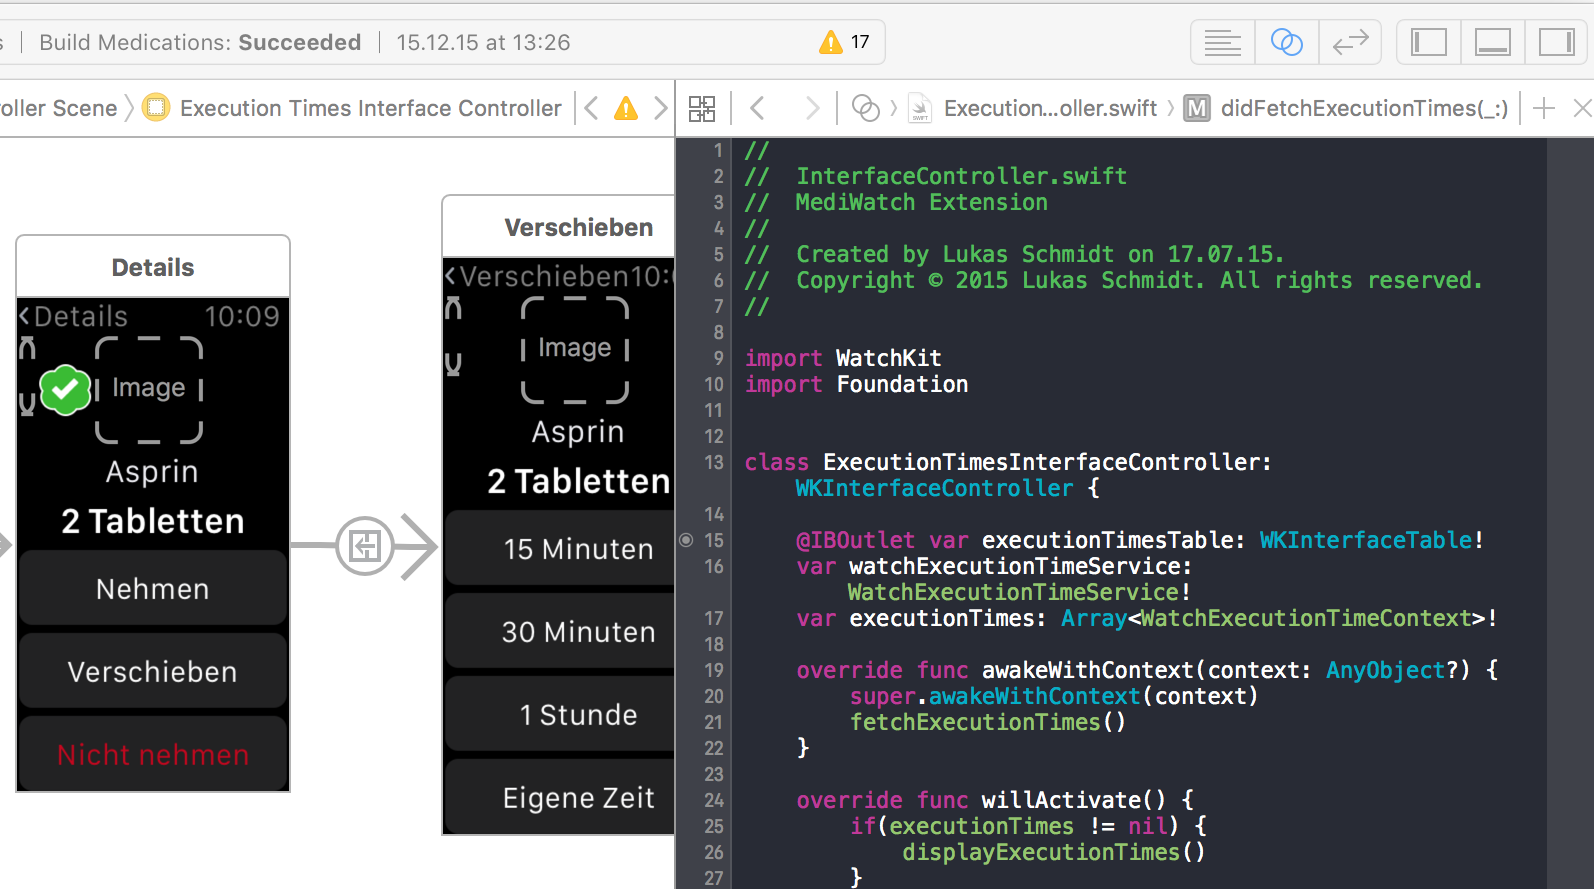
\includegraphics[width=0.9\textwidth]{04_realisation/screenshots/xcode-interface-code-connect}
\end{figure}

\section{WatchConnectivity}
Wichtig für die Kommunikation zwischen Uhr und iPhone ist das WatchConnectivity Framework. Hierbei ist ist im Listing xx zu sehen, wie genau eine Verbindung aufgebaut werden kann. Wichtig ist, das diese Verbindung zum richtigen Zeitpunkt im Application-Lifecycle aufgebaut wird, da es sonst zu Datenverlusten kommen kann. 

Mit der "sendMessage:" Methode können Nachrichten und Datenpakete gesendet werden, welche sich durch eine ID identifizieren lassen. Auch ist möglich eine direkte Antwort auf eine solche Nachricht über einen Replay-Handler zurück zu senden. So kann eine Art Request/Response Datentransfer realisiert werden. Zu beachten ist jedoch, dass die Kommunikation relativ langsam ist. Sie sollte nur verwendet werden um kleine Informationen zu senden.

Werden erst beim Watch-App Start benötigte Daten vom der iPhone angefordert, kann dies zu einer großen Verzögerung kommen. Daher sollten Informationen, die auf der Uhr angezeigt werden, nicht erst zum Zeitpunkt der Darstellung angefordert werden. Gibt es eine Datenänderung auf dem iPhone, die relevante Daten für die Uhr enthält, so sollten diese mit der Methode "transferUserInfo:" an die Uhr gesendet werden. Mit dem Aufrufen dieser Methode wird die übergebene Information nicht direkt zu Uhr geschickt. Das System sendet die Daten zu einem optimalen Zeitpunkt (starke Verbindung zur Uhr, mögliche WLAN Verbindung) an die Uhr. Wenn nun die Watch-App startet, so sind die Daten bereit und können direkt dargestellt werden.

Zum übertragen von größeren Daten steht die Methode "transferFile:" zur Verfügung. Die Methode verhält sich equivalent zu "transferUserInfo:", wird jedoch in der Realisierung nicht verwednet.

\section{Anwendung}

Die Anwendung besteht aus 2 Komponenten auf der Apple Watch. Eine native Notification (\ref{ch:watch_software}). Diese wurde darauf hin optimiert, dass eine große graphische Repräsentation des Medikaments angezeigt wird. Dem Nutzer wird so die Wiedererkennung des Medikaments zu erleichtert (siehe \ref{fig:watch-app-notification}).

\begin{figure}
	\caption{Notification für Medikament}
	\label{fig:watch-app-notification}
	\centering
	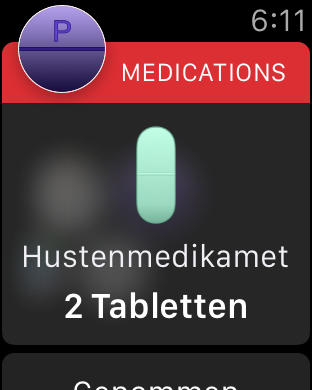
\includegraphics[width=0.5\textwidth]{04_realisation/screenshots/watch/notification.png}
\end{figure}

